\documentclass[sigconf,nonacm]{acmart}

\usepackage{booktabs}
\usepackage{xcolor}
\newcommand{\todo}[1]{\textcolor{red}{[TODO: #1]}}
\newcommand{\ci}[2]{\,[#1,\,#2]}

\settopmatter{printacmref=false}
\renewcommand\footnotetextcopyrightpermission[1]{}

\begin{document}

\title{Scan or Search? Exhaustive LLM Classification versus Agentic Search for Find-All Queries}

% TODO: family names and emails.
\author{Ayesha}
\affiliation{\institution{University of Wisconsin--Madison}\city{Madison}\state{WI}\country{USA}}
\author{Nabanita}
\affiliation{\institution{University of Wisconsin--Madison}\city{Madison}\state{WI}\country{USA}}
\author{Nida}
\affiliation{\institution{University of Wisconsin--Madison}\city{Madison}\state{WI}\country{USA}}

\begin{abstract}
A find-all query asks for every matching document, as in systematic reviews,
legal discovery and audits. An LLM can answer it by \emph{searching}, as an
agent that issues retrieval queries and decides when to stop, or by
\emph{scanning}, asking a yes/no question of every document in large GPU
batches. We compare the two on corpora whose answer sets are complete:
20 Newsgroups, 26 systematic reviews from SYNERGY, and arXiv at up to one
million documents. We express an agent's cost as an exchange rate, the number
of scan decisions one agent step buys on the same GPU: 78 for a 7B agent one
query at a time, 11 with 50 queries batched, and 160--230 for a 32B agent.
Given exactly the agent's time on each query, a scan that reads documents in
embedding order finds more answers than every agent we tried, including a 32B
agent and agents with keyword search, on every dataset. Batching agents closes
the cost gap but not the recall gap. Cheap scorers (BM25, embeddings and
cross-encoder rerankers) are far behind any LLM scan, and the best scan model
depends on the query: open decision models win on short topical and logical
queries, a general instruction model on long eligibility criteria.
\end{abstract}

\maketitle

% ---------------------------------------------------------------------------
\section{Introduction}

Systematic reviews, legal discovery and compliance audits ask for \emph{all}
documents that match a description, and a missed document is the costly error.
LLMs give two ways to answer such \emph{find-all} queries. A search agent wraps
a retriever in a reasoning loop~\cite{yao2023react}: it writes a query, reads
the results, keeps matches and searches again until it decides it is done. It
reads a small part of the corpus, so it is cheap, but it cannot know what it
never retrieved. A scan asks a yes/no question of every document; each decision
is one prefill with no decoding, and decisions batch well~\cite{kwon2023vllm}.
It is complete by construction but costs $O(N)$ model calls. Semantic-operator
systems such as LOTUS~\cite{patel2024lotus} take the scan as their reference
algorithm and make it cheaper; hosted decision models such as
Jev~\cite{typesafe_jev}, and open reproductions~\cite{kev,jev9b}, are built for
it. We ask the question these systems assume: \emph{when is scanning better than
searching?}

We contribute (1)~the \emph{exchange rate}, the scan decisions one agent step
buys on the same GPU, which turns the question into arithmetic; (2)~an
equal-time comparison on three corpora with complete answer sets, four agent
variants and three scan models, in which every scan beats every agent;
(3)~evidence that the answer does not change with corpus size up to one million
documents; and (4)~three negative results: cheap scorers do not replace the LLM,
keyword search makes agents worse, and choosing the scan depth per query does
not beat a fixed depth.

% ---------------------------------------------------------------------------
\section{Setup}

\paragraph{Arms.}
The \emph{scan} asks, for each (query, document) pair, whether the document
matches, and accepts it if $P(\text{yes}) \ge 0.5$ unless stated. The
\emph{agent} sees the request, its previous searches and the top 20 unseen
results as 300-character snippets; it replies with JSON naming the results to
keep and the next search, or stops, for up to 64 steps. Its tool is exact
embedding search (all-MiniLM-L6-v2~\cite{reimers2019sbert}); a variant adds
BM25~\cite{robertson2009bm25} as a second tool and lets the agent choose per
step. Every arm is scored against the complete answer set, so a missed
document always costs recall.

\paragraph{Models.}
Qwen2.5-7B-Instruct~\cite{qwen2025qwen25} serves as both scan (zero-shot,
$P(\text{yes})$ from first-token log-probabilities) and agent, on one vLLM 0.6.3
engine~\cite{kwon2023vllm}, so the main comparison isolates the strategy.
Qwen2.5-32B-Instruct is a stronger agent. Two open decision models,
Kev-9B~\cite{kev} and JEV-9B~\cite{jev9b} (LoRA adapters and a decision head on
Qwen3.5-9B), are alternative scan models. Kev reads the document before the
questions, so one pass over a document can answer every query
(\emph{packed}). All timings are on one NVIDIA H200.

\paragraph{Data.}
\emph{20 Newsgroups}~\cite{lang1995newsweeder}: random subsets of 1K--10K posts
and one query per category; at 10K, answer sets hold 329--555 posts. A
\emph{logic} set adds 25 keyword, AND, OR and NOT queries on the same posts.
\emph{SYNERGY}~\cite{debruin2023synergy}: 26 systematic reviews, each its own
corpus (the 257--48{,}375 records its search returned, all screened; 168{,}946 in
total) with its eligibility criteria as the query and its 9--762 inclusions as
the answer set. Pools are never merged, since a record was screened only for its
own review. \emph{arXiv}~\cite{clement2019arxiv}: a fixed sample of 1M papers
and 20 category queries; a paper is relevant if the category is among its own,
so answer sets (1.4K--59K at 1M) are complete. \emph{NFCorpus}~\cite{boteva2016nfcorpus}
(first 50 queries) is used only for the scorer comparison, since its judgments
are not exhaustive.

\paragraph{Exchange rate and equal time.}
If an agent step takes $\tau$ seconds and the scan classifies $r$ documents per
second, one step buys $E = \tau r$ decisions. To compare at equal cost, we give
the scan exactly the agent's seconds on each query and let it read documents in
embedding order, at its measured rate on that corpus. Scores are saved for every
document (for arXiv, each query's top 20K by embedding), so these plans are
replayed offline. Differences are paired over queries (reviews for SYNERGY) with
95\% bootstrap intervals; tuned thresholds are chosen leaving one query out.

% ---------------------------------------------------------------------------
\section{Results}

\begin{figure*}[t]
\centering
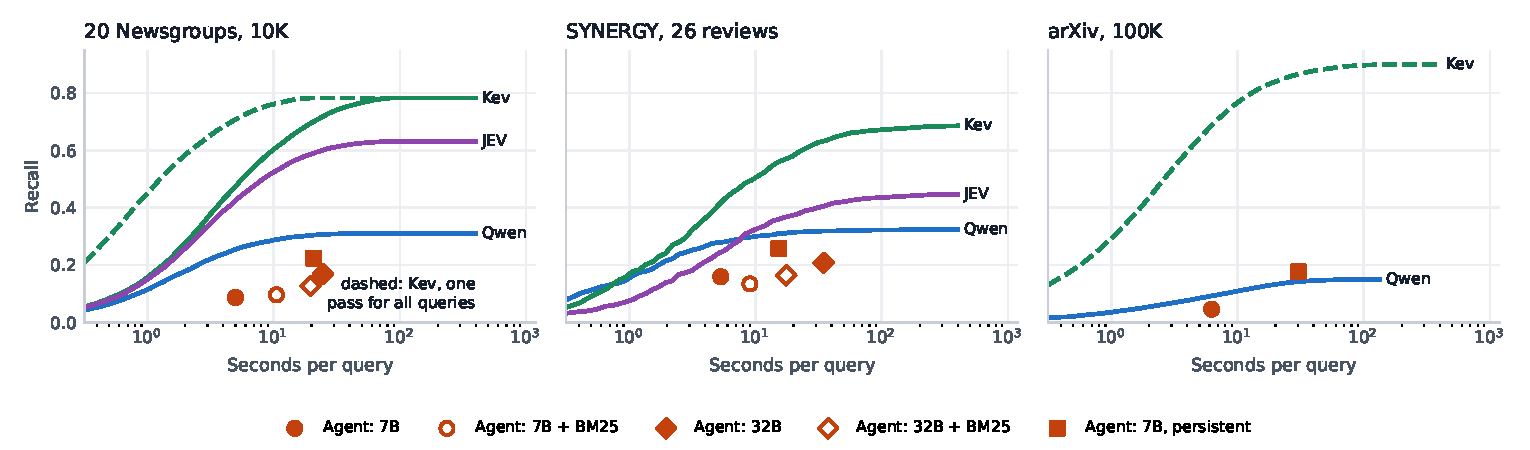
\includegraphics[width=\textwidth]{figs/recall_time.pdf}
\caption{Recall against seconds per query. Curves: each scan model reading
documents in embedding order at its measured rate ($t=0.5$); dashed, Kev with
one pass for all queries. Points: agent variants. Every agent lies below every
scan curve. \todo{arXiv panel.}}
\label{fig:time}
\end{figure*}

\subsection{At equal time, the scan wins}

Figure~\ref{fig:time} and Table~\ref{tab:agents} give the main result. One query
at a time, a 7B agent step costs 0.45\,s, or $E=78$ decisions of the 170 per
second the Qwen scan sustains on 20 Newsgroups. At 10K documents the agent
stops by choice after about 10 steps with recall 0.09; in the same seconds, the
Qwen scan in embedding order reaches 0.22 (+0.14\ci{0.10}{0.18}), JEV 0.38 and
Kev 0.43, or 0.67 when Kev answers all 20 queries in one pass. SYNERGY's long
eligibility criteria slow the scan to 109 documents per second ($E=48$), yet in
the agent's time on each review it still reaches 0.26 against the agent's 0.16
(+0.10\ci{0.05}{0.16}, better on 17 of 26 reviews), and 0.37 with Kev
(+0.21\ci{0.14}{0.28}).

Stronger agents do not change this. The 32B agent with embedding search is the
best agent (0.17 on 20 Newsgroups, 0.21 on SYNERGY), but its steps cost about
1.4\,s ($E \approx 230$ and 160), and given its time the scans reach 0.29--0.68 and
0.32--0.62. Every scan beats every agent on both datasets, and every interval
excludes zero.

\begin{table}[t]
\centering
\small
\setlength{\tabcolsep}{3.5pt}
\begin{tabular}{@{}lrrrrrr@{}}
\toprule
& \multicolumn{3}{c}{20NG 10K} & \multicolumn{3}{c}{SYNERGY} \\
\cmidrule(lr){2-4}\cmidrule(lr){5-7}
Agent & Agent & Qwen & Kev & Agent & Qwen & Kev \\
\midrule
7B & 0.09 & 0.22 & 0.43 & 0.16 & 0.26 & 0.37 \\
7B + BM25 & 0.10 & 0.24 & 0.49 & 0.13 & 0.29 & 0.46 \\
32B & 0.17 & 0.29 & 0.68 & 0.21 & 0.32 & 0.62 \\
32B + BM25 & 0.13 & 0.29 & 0.63 & 0.16 & 0.31 & 0.55 \\
\bottomrule
\end{tabular}
\caption{Recall of each agent, and of the scan given that agent's seconds on
each query ($t=0.5$). JEV, not shown, reaches 0.38--0.57 on 20NG and 0.21--0.40
on SYNERGY.}
\label{tab:agents}
\end{table}

\paragraph{Batching agents.}
A reasoning step is decode-bound, so batching many queries' steps on one GPU
makes each cheaper: with about 53 queries in flight a 7B step costs 0.063\,s,
$E=11$, which is the break-even rate $E^\ast = 11.0$ at which the agent ties the
scan in embedding order. Recall does not move (0.09), and latency rises from
4.5\,s to about 106\,s per query. Batching makes the agent as cheap as the scan,
not as complete.

\paragraph{Keyword search makes agents worse.}
Given BM25 as well as embedding search, agents use it heavily (55--90\% of
searches on SYNERGY) and find less: recall falls from 0.16 to 0.13 (7B) and
from 0.21 to 0.16 (32B) on SYNERGY, and from 0.17 to 0.13 for the 32B agent on
20 Newsgroups. The 7B agent searches twice as long on 20 Newsgroups for the
same recall.

\subsection{Which scorer to scan with}

Table~\ref{tab:scorers} asks whether the scan needs an LLM at all. With the
cutoff tuned on other queries, BM25, embeddings and two cross-encoder rerankers
(bge-reranker-v2-m3~\cite{chen2024bgem3} and ms-marco-MiniLM-L6-v2) trail every
LLM scan on 20 Newsgroups, the logic queries and SYNERGY. The rerankers are
7--11$\times$ faster than the Qwen scan but rank no better than plain
embeddings. Only on NFCorpus, whose judgments are incomplete, does zero-shot
Qwen merely tie BM25.

Which LLM is best depends on the query. On short topical and logical queries,
both decision models beat zero-shot Qwen: on the logic set F1 rises from 0.58 to
0.77 (Kev) and 0.79 (JEV), and at $t=0.5$ NOT queries from 0.18 to 0.63--0.70.
Their best threshold is 0.3--0.9 on 20 Newsgroups, the logic set and NFCorpus,
while Qwen's ranges from $10^{-8}$ on 20 Newsgroups to 0.9 on NFCorpus. On SYNERGY's long, multi-condition criteria,
zero-shot Qwen ranks as well (AP 0.36 against 0.38 and 0.34) and has the best
tuned F1 (Kev $-0.10$\ci{-0.17}{-0.05}). For screening, Qwen also leaves the
most work saved at 95\% recall (WSS@95~\cite{cohen2006wss} 0.58).

\begin{table}[t]
\centering
\small
\setlength{\tabcolsep}{3.2pt}
\begin{tabular}{@{}lrrrrrrr@{}}
\toprule
& BM25 & Emb. & bge & MiniLM & Qwen & Kev & JEV \\
\midrule
20NG 10K & 0.37 & 0.48 & 0.35 & 0.29 & 0.58 & \textbf{0.65} & 0.63 \\
Logic 10K & 0.32 & 0.31 & 0.23 & 0.18 & 0.58 & 0.77 & \textbf{0.79} \\
NFCorpus & 0.16 & 0.12 & 0.13 & 0.15 & 0.12 & 0.18 & \textbf{0.20} \\
SYNERGY & 0.11 & 0.15 & 0.10 & 0.13 & \textbf{0.32} & 0.22 & 0.25 \\
\midrule
Docs/s & -- & -- & 1,138 & 1,879 & 170 & 121 & 127 \\
\bottomrule
\end{tabular}
\caption{F1 with the cutoff tuned on other queries. Throughput is per query on
20 Newsgroups; Kev reaches 540 when one pass answers all 20 queries.}
\label{tab:scorers}
\end{table}

\subsection{Scale}

\todo{arXiv at 10K, 100K and 1M: agent recall and seconds, scan recall in the
agent's time, and how both change with N. A full scan of 1M documents at 170
documents per second takes about 98 minutes per query.}

\subsection{What did not help}

\paragraph{Choosing the depth per query.}
A hybrid that classifies the top $k$ by embedding is an access-path choice. Four
rules that set $k$ per query (score mass, the largest similarity gap after
\cite{taguchi2025adaptivek}, answer-size estimates from a random sample, and
stopping when the acceptance rate falls) tie or lose to a fixed $k$ at equal
mean cost. An oracle that sees the answers adds only 0.01--0.07 recall, because
$k$ must follow $N$ more than the query, in line with Meng et
al.~\cite{meng2024rlt} for re-ranking depth.

% ---------------------------------------------------------------------------
\section{Related Work}

Ranked list truncation learns where to cut a ranking~\cite{bahri2020choppy,
wu2021attncut}; for LLM re-ranking, supervised cut-offs show no clear advantage
over a fixed depth~\cite{meng2024rlt}. Technology-assisted review studies when
human screening can stop~\cite{cormack2016tar,yang2021stopping}. LOTUS
\cite{patel2024lotus} and Kim et al.~\cite{kim2026semfilter} make semantic
filters cheaper with proxy-model cascades that keep accuracy targets; our scan
is their reference algorithm, and cascades would lower our scan costs further.
We instead compare the scan with the agentic alternative.

% ---------------------------------------------------------------------------
\section{Conclusion}

For find-all queries, scanning beats searching whenever an agent step costs more
than about a dozen classifier decisions. On one GPU a step costs 48--230 of them
one query at a time, depending on the agent and the corpus. Batching agents closes the cost gap but not the
recall gap, a larger agent costs more than it gains, and keyword search hurts.
\emph{Limitations:} one GPU type; a single agent design; 20--26 queries per
dataset; SYNERGY inclusions were decided on full text, which caps every arm;
and Kev and JEV use a different, larger backbone than Qwen.

\bibliographystyle{ACM-Reference-Format}
\bibliography{refs}

\end{document}
